\documentclass[a4paper]{article}

% natbib
\usepackage[numbers,sort]{natbib}

\usepackage{mysimpletemplatewn}
\usepackage[utf8]{inputenc} %%% to support copy and paste with accents for french stuff
\usepackage[T1]{fontenc} %%%key to get copy and paste for the code!
\usepackage{times}
\usepackage[french]{babel}
\usepackage[scaled=0.85]{helvet}
\usepackage{graphicx}
\usepackage{ifthen}
\usepackage{xspace}
\usepackage{alltt}
\usepackage{latexsym}
\usepackage{url}
\usepackage{amsmath,amssymb,amsfonts}
\usepackage{stmaryrd}
\usepackage{algorithmic}
\usepackage{textcomp}
\usepackage{xcolor}
\usepackage{enumerate}
% \usepackage{cite}
\usepackage[pdftex,colorlinks=true,pdfstartview=FitV,linkcolor=blue,citecolor=blue,urlcolor=blue]{hyperref}
\usepackage{multirow}
\usepackage{listings}
\usepackage{color}
\usepackage{subcaption}

\usepackage{pgfgantt}

\usepackage{bibentry}
\nobibliography*


\newboolean{showcomments}
\setboolean{showcomments}{true}
\ifthenelse{\boolean{showcomments}}
  {\newcommand{\bnote}[2]{
	\fbox{\bfseries\sffamily\scriptsize#1}
    {\sf\small$\blacktriangleright$\textit{#2}$\blacktriangleleft$}
    % \marginpar{\fbox{\bfseries\sffamily#1}}
   }
   \newcommand{\paragraphDesc}[2]{
    \textcolor{#1}{#2}
   }
   
  }
  {\newcommand{\bnote}[2]{}
   \newcommand{\cvsversion}{}
   \newcommand{\paragraphDesc}[2]{}
  }

\newcommand{\here}{\bnote{***}{CONTINUE HERE}}
\newcommand{\nb}[1]{\bnote{NB}{#1}}

\newcommand{\fix}[1]{\bnote{FIX}{#1}}
%%%% add your own macros 


\newcommand{\sd}[1]{\bnote{Stef}{\textcolor{orange}{#1}}}
\newcommand{\an}[1]{\bnote{Anne}{\textcolor{green}{#1}}}
\newcommand{\bv}[1]{\bnote{Benoit}{\textcolor{blue}{#1}}}
\newcommand{\nic}[1]{\bnote{Nic}{\textcolor{red}{#1}}}

\newcommand{\todo}[1]{\bnote{TODO}{#1}}

\graphicspath{{figures/}}
%%% 


\newcommand{\figref}[1]{Figure~\ref{fig:#1}}
\newcommand{\figlabel}[1]{\label{fig:#1}}
\newcommand{\tabref}[1]{Table~\ref{tab:#1}}
\newcommand{\layout}[1]{#1}
\newcommand{\commented}[1]{}
\newcommand{\secref}[1]{Section~\ref{sec:#1}}
\newcommand{\seclabel}[1]{\label{sec:#1}}

%\newcommand{\ct}[1]{\textsf{#1}}
\newcommand{\stCode}[1]{\textsf{#1}}
\newcommand{\stMethod}[1]{\textsf{#1}}
\newcommand{\sep}{\texttt{>>}\xspace}
\newcommand{\stAssoc}{\texttt{->}\xspace}

\newcommand{\stBar}{$\mid$}
\newcommand{\stSelector}{$\gg$}
\newcommand{\ret}{\^{}}
\newcommand{\msup}{$>$}
%\newcommand{\ret}{$\uparrow$\xspace}

\newcommand{\myparagraph}[1]{\noindent\textbf{#1.}}
\newcommand{\eg}{\emph{e.g.}\xspace}
\newcommand{\ie}{\emph{i.e.}\xspace}
\newcommand{\etal}{\emph{et al.,}\xspace}
\newcommand{\ct}[1]{{\textsf{#1}}\xspace}
\newcommand{\etc}[1]{\textit{etc.}}



\newcommand{\defaultScale}{0.55}
\newcommand{\pic}[3]{
   \begin{figure}[h]
   \begin{center}
   \includegraphics[scale=\defaultScale]{#1}
   \caption{#2}
   \label{#3}
   \end{center}
   \end{figure}
}


\newcommand{\twocolumnpic}[3]{
  \begin{figure*}[!ht]
  \begin{center}
  \includegraphics[scale=\defaultScale]{#1}
  \caption{#2}
  \label{#3}
  \end{center}
  \end{figure*}
}

\newcommand{\picw}[3]{
  \begin{figure}[htbp]
  \begin{center}
  \includegraphics[width=\columnwidth]{#1}
  \caption{#2}
  \label{#3}
  \end{center}
  \end{figure}
}


\newcommand{\infe}{$<$}
\newcommand{\supe}{$\rightarrow$\xspace}
\newcommand{\di}{$\gg$\xspace}
\newcommand{\adhoc}{\textit{ad-hoc}\xspace}

\usepackage{url}            
\makeatletter
\def\url@leostyle{%
  \@ifundefined{selectfont}{\def\UrlFont{\sf}}{\def\UrlFont{\small\sffamily}}}
\makeatother
% Now actually use the newly defined style.
\urlstyle{leo}

\definecolor{codegreen}{rgb}{0,0.6,0}
\definecolor{codegray}{rgb}{0.5,0.5,0.5}
\definecolor{codepurple}{rgb}{0.58,0,0.82}
\definecolor{backcolour}{rgb}{0.95,0.95,0.92}

\lstdefinestyle{mystyle}{
    backgroundcolor=\color{backcolour},
    commentstyle=\color{codegreen},
    keywordstyle=\color{magenta},
    numberstyle=\tiny\color{codegray},
    stringstyle=\color{codepurple},
    basicstyle=\footnotesize,
    breakatwhitespace=false,
    breaklines=true,
    captionpos=b,
    keepspaces=true,
    numbers=left,
    numbersep=5pt,
    showspaces=false,
    showstringspaces=false,
    showtabs=false,
    tabsize=2
}

\lstset{style=mystyle}
\newcommand{\browserMaster}{\textit{BrowserMaster} \xspace}

\title{CST --Analyse multi-facettes et opérationnelle pour la transformation des systemes d’information}
\author{ HOUEKPETODJI Mahugnon Honoré}

\begin{document}

\institution{}

\date{\today}

\maketitle

% \begin{abstract}
% The abstract text goes here.
% \end{abstract}

\section{Description du sujet de la thèse}
% 0.5 (1/2) pages
CIM est une SAS au capital social de 200k détenu a 100 par DL Software. 
CIM est éditeur, intégrateur, hébergeur et infogéreur de solutions pour l'assurance de personnes en santé, prévoyance. 
Elle offre une expertise Santé et Prévoyance acquise après plus de 30 ans auprès de ses clients. 
CIM est hébergeur de ses solutions pour 90 de ses clients et plus de 1000 utilisateurs. 
Toutes les thématiques d'infrastructure et de surveillance des flux sont intégrées à cette offre.
CIM est propriétaire de ses infrastructures serveurs, tous les éléments actifs des systèmes et tous les éléments de stockage sont achetés par CIM, gérés et supervisés par les équipes de CIM. Aucun sous-traitant n'intervient dans les opérations quotidiennes d'hébergement, d'exploitation des solutions et des données hébergées.

CIM est certifiée Microsoft GOLD Partner. 
Elle est l'éditeur des progiciels de la gamme Izy Links et assure l'intégration de l'ensemble des briques de cette gamme ainsi que des briques partenaires nécessaires à la bonne réussite du projet. Cette solution est développée en PowerBuilder sur base de données DB2. L'équipe de développement
vient d'upgrader en PowerBuilder 2017 (été 2018) et est en cours de passage sur DB2 v11 (avec l'aide d'un DBA IBM – prestation 2018).

Le système de gestion est centré sur le back office Izy Protect, autour duquel gravite l'ensemble des briques complémentaires répondant à l'assemble des besoins, et pouvant
être activées ou non. 
La société CIM a effectué une analyse de risque pour son évolution et croissance en 2017 d'où il ressort que Izy Protect souffre des problèmes 
(1) vieux langage,
(2) logiciel vieillissant,
(3) perte savoir,
(4) changements à haut risque.
Ces problèmes sont récurrents chez les organises gérant des systèmes d'information \cite{Deme02a}.

Ce travail de doctorat consiste de proposer des modèles et des mécanismes permettant d'assurer
une ré-ingénierie des systèmes d'information. Les expériences et validation des prototypes se feront dans le contexte de l'application du système d'information écrit en PowerBuilder de la société CIM
\section{Etat de l'art}
\label{sec:stateOfTheArt}
% 1 pages

Cette section présent Izy Protect, ainsi que les mécanismes de ré-ingénierie des systèmes d'information patrimoniaux.
\subsection{Présentation de Izy Protect}
\label{sec:izyProtect}
Izy Protect est un système de plus de 3 MLOC écris en Powerbuilder et maintenu depuis plus de 20 ans par les développeurs la CIM. Le code source est organisé par bibliothèques Powerbuilder. 
Izy Protect compte 117 bibliothèques. La plus large  à une taille supérieur à 300 KLOC.
Durant toutes ces années, il y a eu beaucoup de changement dans l'equipe de developpeurs.  
Vu la complexité actuelle du système, les développeurs ont de plus en plus du mal a le maintenir.
 Les ancienne versions du système sont stocker sur un disque dure. Pour des raison interne à la CIM, les versions de Izy protect ont été perdu jusqu'en 2010.  De plus les développeurs risquent a tout moment d'écraser leurs travaille. Les développeurs modifient Izy protect en réponse a qui décrit le travaille a faire. 
De plus, il n'y a pas de tests unitaire automatisés.
Ce qui augment la craint des développeurs au petit changement. 
Quand un système à plusieurs décennie de vie, la retro-ingénierie est une activités centrale pour le maintenir \cite{Deme02a}.

Dans l'entreprise, les tickets sont stockés dans la base de données des tickets ou fiches navettes depuis 1998. 
Un ticket représente un travail unitaire.
La base de données des tickets pilote l'ensemble du processus d'évolution du logiciel : attribution du travail aux développeurs, gestion du flux de travail pour répondre à une demande du client, informations de facturation sur chaque tâche.
Il existe des tickets pour la correction de défauts, la rédaction de documentation, l'ajout de nouvelles fonctionnalités, etc. 

Un ticket comporte entre autres les caractéristiques suivantes:

\begin{itemize}
\item  la date de création
\item la date de clôture
\item l'estimation du temps nécessaire au développeur pour travailler sur le ticket
\item temps passé par un développeur
  \begin{itemize}
  \item le temps d'analyser
  \item le temps de mettre en œuvre une solution
  \item le temps de test
  \end{itemize}
  \item le(s) bibliothèque(s) impactées
\end{itemize}

\subsection{Analyse de l'évolution de l'état d'un logiciel patrimonial}
\label{sec:etatLogiciel}

Les systèmes  patrimoniaux sont des systèmes en constante changements: production de nouvelles fonctionnalités.
 La deuxième loi de Lehman \cite{Lehm96a} stipule qu'à mesure que les logiciels évoluent, la complexité croissante et l'augmentation des défauts entraîneront une baisse de la satisfaction des parties prenantes, à moins que les équipes de projet n'entreprennent le travail nécessaire pour maintenir la qualité.
 Dans ce sens nombreuses travaux de la littérature propose des techniques, pour suivre l'évolution de l'état de  ces systèmes.
 
\citep{Zhan10b} utilise les données des occurrences bugs et le temps pour modéliser l'évolution d'un système logiciel avec  c\-charts.

\citep{lenar17} propose un système de recommandation  d'action au développeur pour un nouveau bug. Le system se  base sur l'historique des bugs, le code source ainsi que qu'un algorithme de prédiction.  Pour que ça marche, le code source doit être gérer dans un système de contrôle de version. Ce qui n'est pas le cas avec Izy Protect.
 
\citep{port17} utilise les modèles  et l'analyse de l'historique des défauts pour évaluer la qualité d'un système et prédire l'effort nécessaire pour améliorer le système. Les métriques mesurés sont: le taux de bugs sur une période de temps, le ratio entre le taux de d'augmentation de la taille du système et le taux de bugs, le temps moyen entre la découverte des bugs, l'effort pour résoudre les bugs, estimation des risque de future bugs, etc.
 Certain de ces métriques comme: le taux de bugs par période de temps, l'effort pour résoudre les bugs  sont intéressantes dans le cadre de Izy Protect. 
Les autres ne se conforme pas au contexte car les tickets de Izy protect ne sont directement liés au code de façon standard.
Chaque développeur note le numéro de tickets a sa façon dans le code. 
 

\cite{kim07,Bibi06} propose  un modèle de prédiction des défauts avec des algorithmes d'apprentissage en utilisant l'historique des bugs de système. 
Les algorithmes de prédiction de bugs ne sont pas toujours consistant \cite{bang19}. De plus, ils ne tiennent pas compte des changements qui peuvent être imprévisible dans le code. De plus Izy Protect est système commercial multi-utilisateurs, et donc chaque utilisateur a des fonctionnalités ou des changements qui lui est spécifique. 

\cite{naga05} Utilise l'historique le nombre de lignes de code changer pour un bug fix ou une nouvelle fonctionnalité pour prédire la densité de bug  le code. Pour que ceci soit réalisable, il faut que le code soit préalablement versionné dans un system de contrôle de version.

\cite{Raja09} à étudier différents algorithme de modélisation des défauts d'un système a partir des donnée des défauts relevé sur huit projet open source. Il en ressort que la moyenne glissée modélise mieux les défauts des systèmes.

\subsection{Rétro-ingénierie}
\label{sec:retroingenierie}
Dans cette section, je presenterais  les traveaux reliés à outillage pour la rétro-ingénierie que j'ai étudié.
\cite{Chik90a} définit la rétro-ingénierie comme \textit{"un proccessus 
 d'analyse d'un système donnée pour identifier les composants du système et leurs relations,
afin de créer des représentations du système sous une autre forme ou à un niveau d'abstraction plus élevé."}.

\cite{Brun14c} afirme que la rétro-ingénierie  n'est pas limitée à certains langages courants 
 mais est universelle. 
Par exemple, elle peux concerner  la base de données \citep{Delp20a} ou  l'interface graphique \citep{Verh19a}.
Il est donc nécessaire de disposer d'une suite d'outils polyvalents et extensibles, indépendants du langage : cette extension peut se faire à plusieurs niveaux - méta-modèle.
Mais aussi au niveau des outils eux-mêmes (par exemple en agissant sur le modèle).

Kienle et Müller \cite{Kien10a} ont explorer la question de la construction d'outils de rétro-ingénierie.
 Ils proposent trois axes : (1) les critères, (2) la construction et (3) l'évaluation.

Bellay et Gall \cite{Bell98a} ont proposé une large liste de critères pour comparer les outils de rétro-ingénierie.
Par contre ils ne couvrent  pas le métamodèle, l'extension du métamodèle et des outils de manière exhaustive.

Govin et al \cite{Govi18a} ont identifié des critères pour les outils de  réingénierie. 
Parmis ces critères  j'ai retenu ceux qui rapportent à la rétro-ingénierie.
Ce sont les critères (1) de selection , (2) d'abstraction. 

%Modisco
\citet{Brun14c} a proposé et mis en oeuvre le cadre MoDisco.
MoDisco est divisé en 4 couches, le projet de modélisation des éclipses, l'infrastructure, la technologie et les cas d'utilisation.
La couche infrastructure contient des outils génériques tels que celui permettant de naviguer et d'interroger les modèles.
La couche technologie contient le métamodèle spécifique, (Java, XML, JSP, ...).
Et la couche des cas d'utilisation contient l'action spécifique pour un modèle, par exemple le refactoring de code Java. 
MoDisco inclut , navigateur de model, un editeur pour voir le code des entité d'un model, un support graphique pour faire des requetes sur les elements du model. 
Par contre \citet{Brun14c}, ne propose que l'UML pour visualiser les elements d'un model.
Alors que pour un système large, l'UML devient vite une toile d'araigné et fraine une compréhension rapide du système.


\section{Avancées actuelles}
% 3 pages
\subsection{Route vers le DevOps}
\label{sec: devOps}
Les problèmes préalablement cités sur Izy Protect à savoir: code non versionné, ce qui engendre les pertes et écrasement de code, puis l'absence total de test unitaire automatisé, m'ont amenés à:
\begin{itemize}
\item Mettre en place un serveur subversion (SVN) pour versionné les code. 
Le choix de SVN est guidé par le fait  de sa simplicité  pour la compréhension.  
De plus le module de contrôle de version que offre Powerbuilder n'est pas trop stable. 
Par exemple parfois le module considère un code déjà versionné comme un code non versionné.
 De plus le module de contrôle de version que offre Powerbuilder ne support pas bien les opérations avancés comme la comparaison de deux versions du code ou bien la résolution de conflit. En complément de Powerbuilder,  j'ai amener les développeurs de la CIM à utiliser TortoiseSVN.
\item Reconstruire l'histoire du code source de Izy Protect depuis 2012 afin de procéder à des analyse de l'évolution du système a partir des changements entre les version. Les versions de Izy Protect sont nombreuses. J'en suis actuellement a fin des versions produites en 2014.
\item Tester  des outils de tests unitaire sur Powerbuilder. PBUnit parait être la librairy qui permet de tester  les fonctionnalités des applications Powerbuilder au niveau du code source. 
Je suis entrain de le mettre en place.
\end{itemize}

\subsection{Analyse des fiches navettes}
\label{sec:analyseDesFichesNavettes}
Afin d'évaluer l'état de Izy Protect, et contrôller l'effet de la ré-ingénierie sur Izy Protect,
 j'ai utilisé la base de donnée des fiche navettes. 
Après nettoyage, seul les tickets à partir de 2004 sont utilisable. 
Les données sont non-stationnaires. 
En me basant sur les résultats de \cite{Raja09}, j'ai utilisé la moyenne glissant avant un pas de 2 mois pour modéliser l'état du système.
J'ai principalement mesuré les métriques suivantes: l'evolution du temps pour ferme les tickets, l'evolution du temps néccéssaire au developpeur, l'evolution du temps des tests manuel du developpeur,
l'évolution de l'estimation du temps de developpement par le manager.
Les resultats sont presenté dans un dashboard qui se met a jours chaque mois.
La \figref{dashboardFig} montre l'apperçu du dashboard.
Les developpeurs ont confirmés que les resultats de l'analyse reflètent bien leurs ressentit de l'état de Izy Protect. 

\begin{figure}[htbp]
  \begin{center}
  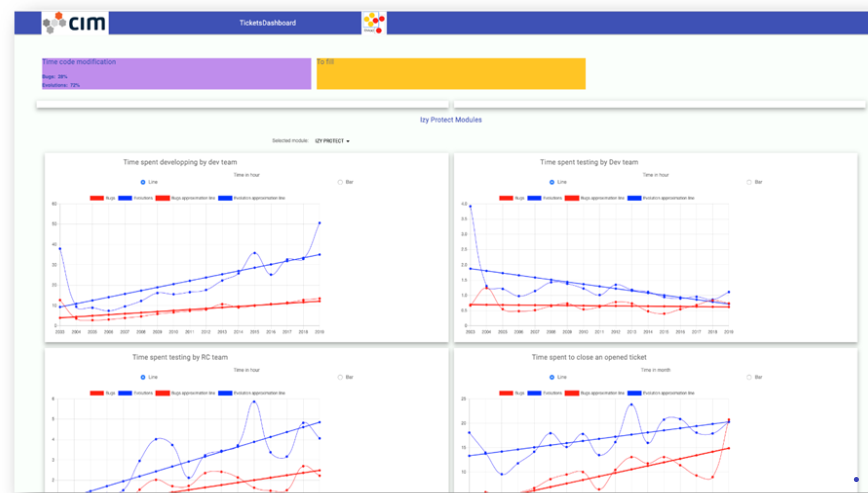
\includegraphics[width=\textwidth]{./figures/dashboard.png}
  \caption{Dashboard d'analyse de tickets}
  \label{fig:dashboardFig}
\end{center}
\vspace{-0.3cm}
\end{figure}


\subsection{Outil d'aide a la rétro-ingénierie logiciel}
Pour répondre aux exigences détaillées dans la section \secref{retroingenierie}, j'ai développé une suite d'outils d'aide à la retro-ingenierie.
Ces outils sont developpeur au dessus de la platform Moose \cite{Nier05c}.
En effet, la plate-forme offre un méta-modèle générique et quatre outils principaux pour l'analyse des systèmes logiciels.
Il s'agit de (1) Famix: un meta-model qui permet au developpeur de representer un programme, (2) Moose Query: un API pour naviguer dans un model Famix,
(3) Les tags: utilisées pour enrichir le code source avec des informations qui ne peuvent pas être directement déduites du code source et 
(4) Roassal: Un framework de visualisation intégré dans Moose.
Dans la suite, je presenterai d'abord l'achitecture mise en place pour les outils puis  chaque outils.


\subsubsection{Architecture des outils }
\begin{figure}[htbp]
  \begin{center}
  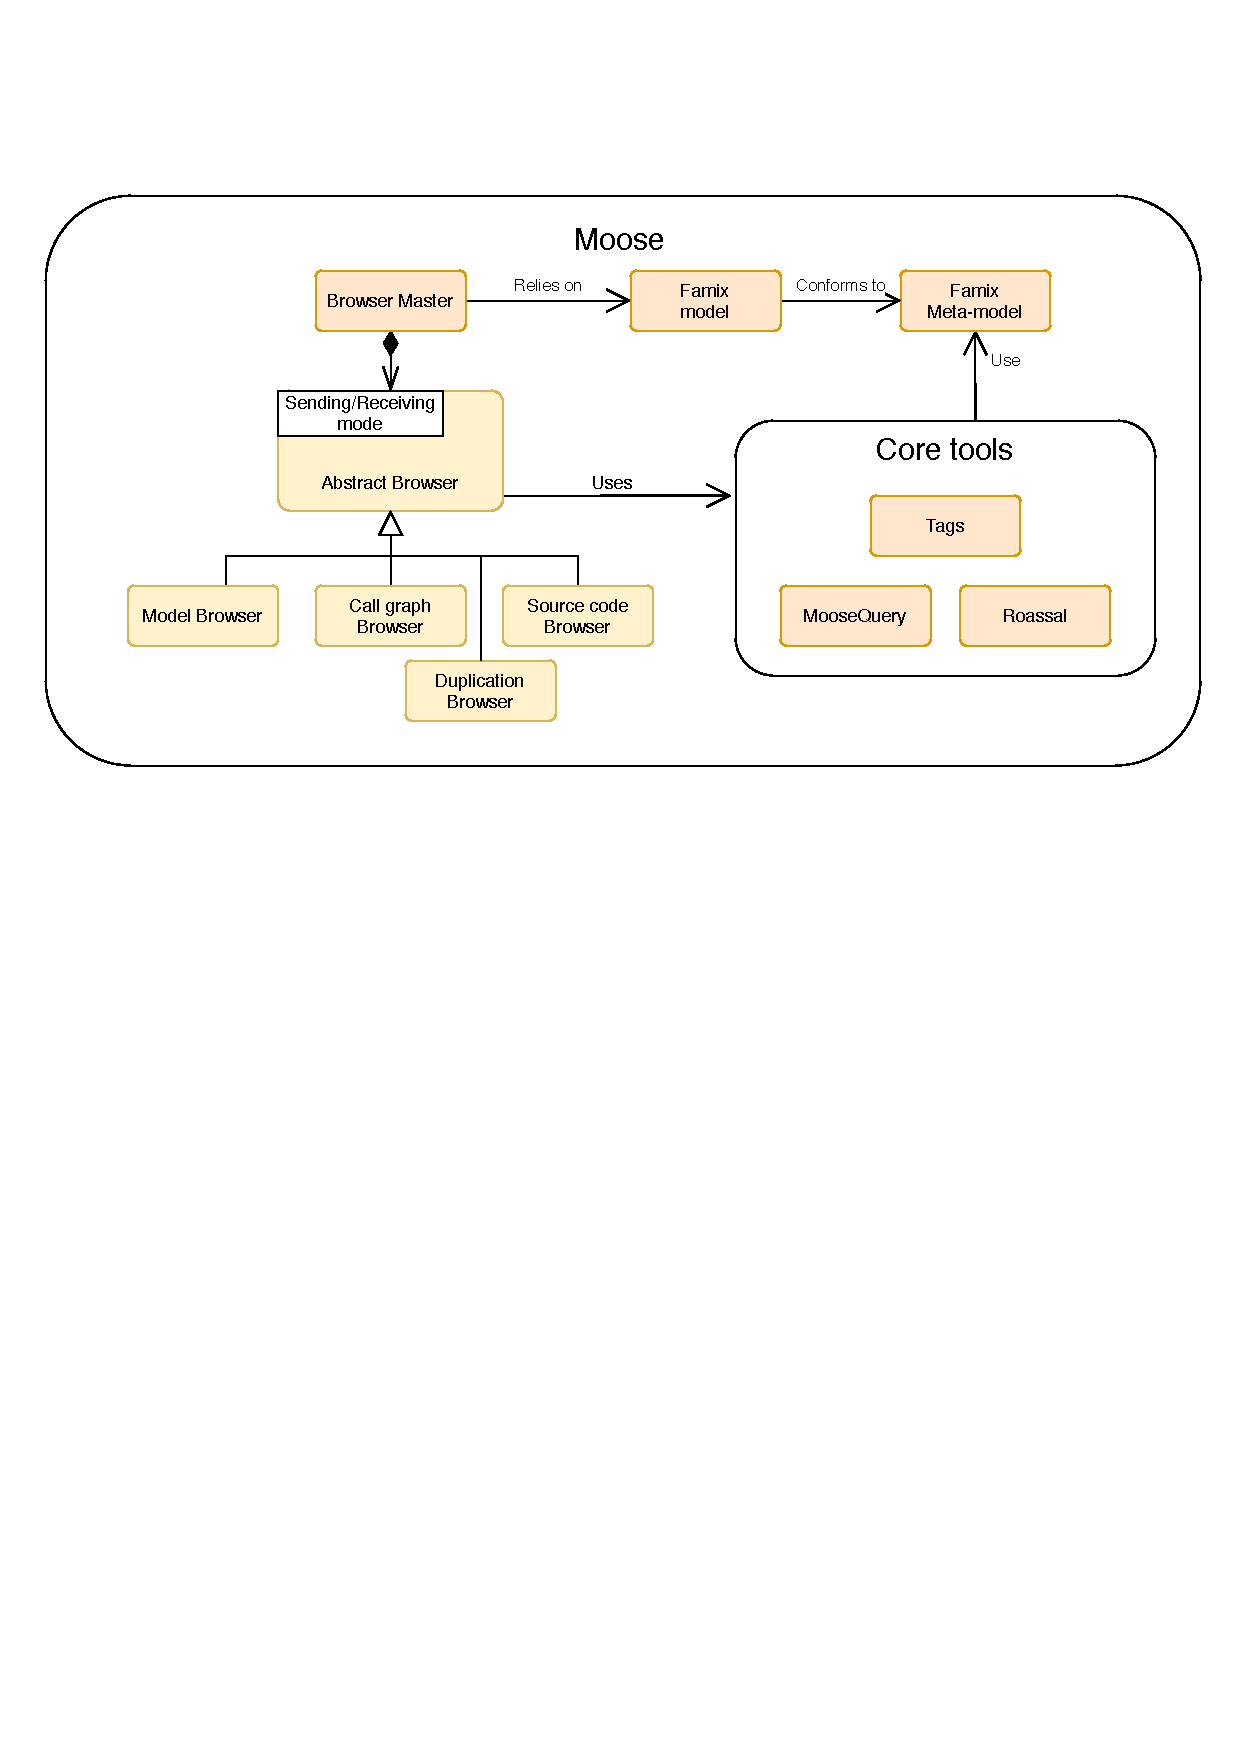
\includegraphics[width=0.7\linewidth]{./figures/architecture.pdf}
  \caption{Architecture de la suite d'outils}
  \label{fig:applicationArchitecture}
  \end{center}
  \vspace{-0.3cm}
\end{figure}

La \figref{applicationArchitecture} montre l'architecture globale de la suite d'outils.
L'architecture global  de la suite d'outils est principalement composé d'un \browserMaster et des navigateurs.
Le tout s'execute sur une instance d'un model Famix. 
Il a été pensé dans le but de facilité l'experience du developpeur dans les differentes activités de la retro-ingenierie logiciel.
Le \browserMaster est responsable de l'exchange d'information entre les navigateurs.
Il est au courant de tous les navigateurs ouvert. 
Il se charge de notifier tous les navigateurs ouvert en cas d'évènement.

Chaque navigateur fonction sur une entité du model Famix  local a lui.
Cet entité peut être un seul entité ou un group d'entité.
Il navigateur est peut émettre ou recevoir un evenement. 
\paragraph{emission d'évènement:} L'emission d'un evènement par un navigateur est gouverner par son mode de propagation.
En mode de propagation actifs, le navigateur emet un evenement pour publier  son entité courant a chaque fois que l'entité change.
Dans le contraire, l'entité courant est gardé localement.

\paragraph{reception d'évènement: } Le comportement d'un navigateur a la reception d'un évènement dépend du mode de réception de ce dernier.
Ainsi chaque navigateur possède trois mode de réception d'évènement. 
Il s'agit des modes (1) \textit{follow}: le navigateur change remplace son entité courant par l'entité reçu via l'evènement,
(2) \textit{highlight}: le navigateur cherche l'entité reçu via l'évènement dans son entité courant, s'il le trouve, il le colorie,
(3) \textit{ignore}: le navigateur ne fait rien a la reception de l'évènement.

Tous les navigateurs presentents un boutton qui indique sont mode d'émission d'évènement, et tois bouttons qui indiquent sont mode de reception d'évènement
\subsubsection{Nivagateur de model}
\begin{figure}[htbp]
  \begin{center}
  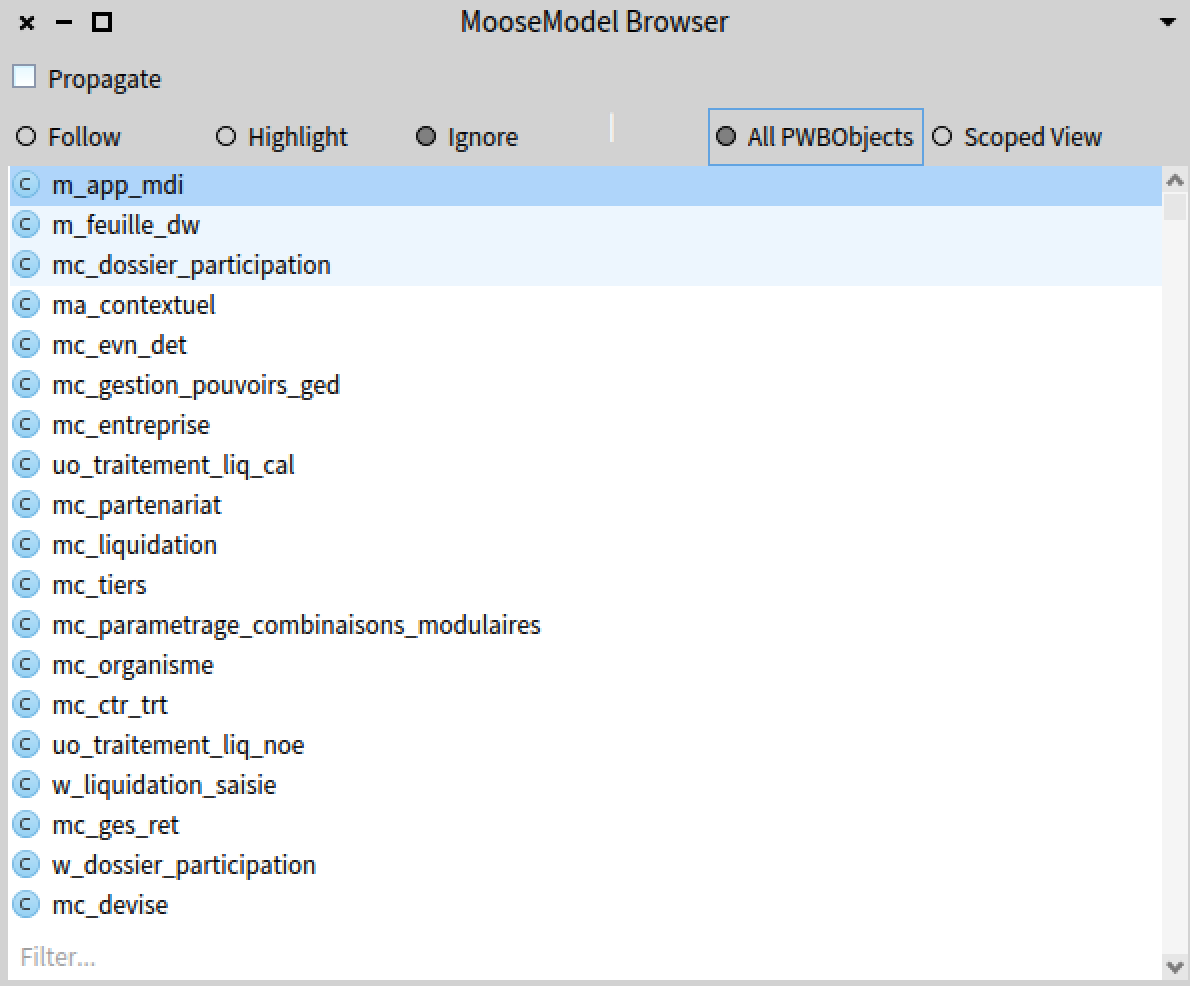
\includegraphics[width=0.5\textwidth]{./figures/modelBrowser.png}
  \caption{Navigateur de model}
  \label{fig:modelBrowser}
\end{center}
\vspace{-0.3cm}
\end{figure}
 Le navigateur de model comme le montre la \figref{modelBrowser} outre la partie commune a touts les navigateurs, comporte deux bouttons (\textit{All PWBObjects}, \textit{Scoped View}), un contenu et un champ de recherche.
 
Le contenu navigateur presente par défaut la liste des entités que contient l'éntité courant du navigateur. 
L'utilisateurs peut décidé de se concentrer sur un certain nombres d'entité. Dans ce cas il les selectionne et il active le boutton  \textit{Scoped View}.
Pour le moment le navigateur de model est juste une liste. Mais Il est prévu de l'étendre.

Le champ de recherche du navigateur permet à l'utilisateur d'écrire une requête de recherche sur son entité Famix courante.
 Cette entité est pour la plus part du temps un groupe d'entité Famix.
Cette requête peut être lexicale, sous forme de simple chaîne pour une recherche lexicale, ou structurelle.
Par exemple, si l'utilisateur recherche \textit{include : FamixPWBAttribute}, le résultat sera toutes les entités contenant des FamixPWBAttribute (attributs Powerbuilder).

\subsubsection{navigateur de graph d'appel}
\begin{figure}[htbp]
  \begin{center}
  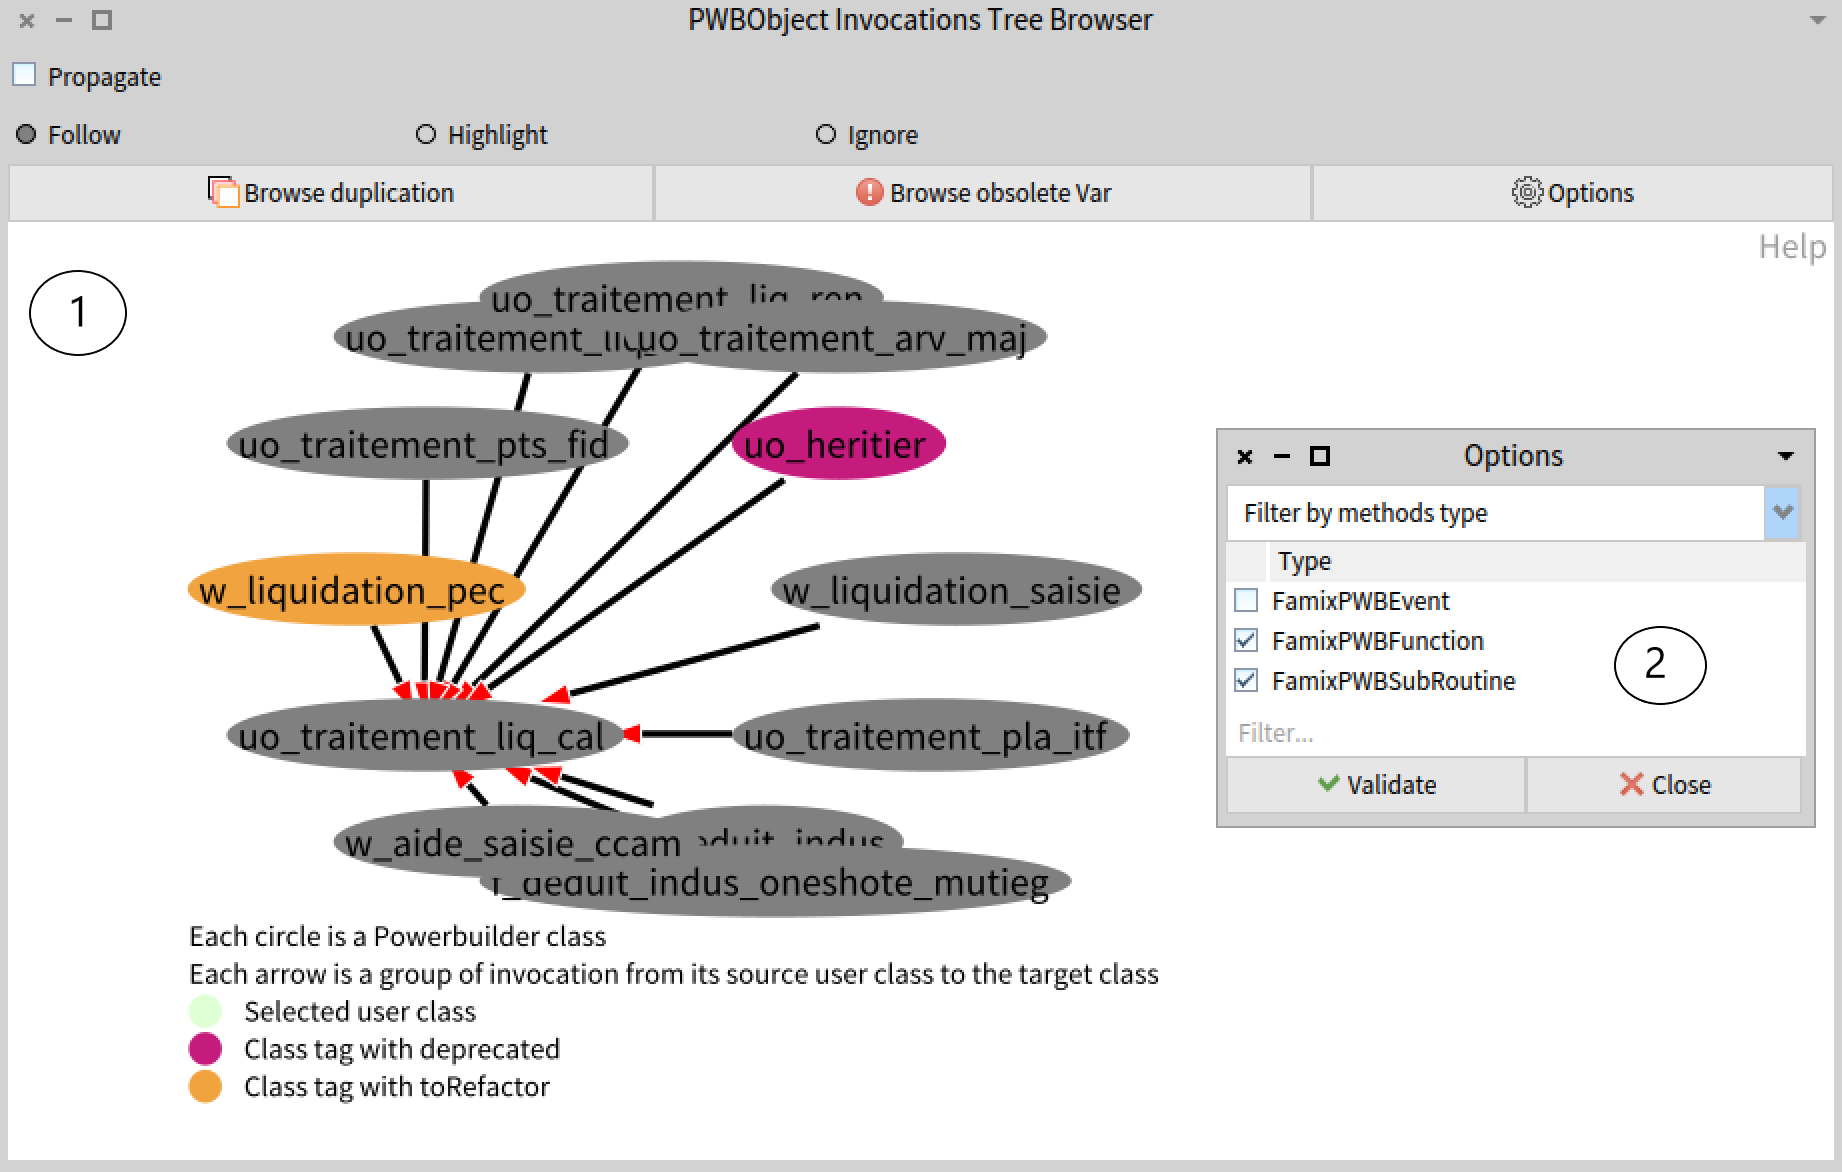
\includegraphics[width=0.7\textwidth]{./figures/callGraphBrowser.png}
  \caption{Graphe d'appel avec l'option de reduction de complexité du graphe}
  \label{fig:graphAppel}
\end{center}
\vspace{-0.3cm}
\end{figure}
La \figref{graphAppel} donne un apperçu du graphe d'appel avec les options. 
Ce outil permet principalement de visualizer sous forme d'un graph les entités qui utilisent l'entité courant du navigateur.
Les noeuds reprensentent les entités. Les fleches reprensentent l'ensemble des utilisations entre deux entités.
Le sens de la flèche indique le sense des utilisations.
En effet pour un système large comme Izy Protect par exemple, ce graph peut rapidement devenir illisible. 
Pour palier a ce problème, l'outil integre un panel d'option qui permet de fitrer le graph par type d'entité a l'origine des appelles.
Afin de donner plus de contexte au developpeur, quand  il glisse la souris sur une flèche,  un popup lui montre toutes les utilisationsavec leurs code source.

Le navigateur de graph d'appel pemet aussi au developpeur de marquer les entités afin de lui ajouter une information qu'on ne peux pas extraire directement du code source.
Une connaissance qui ressort de l'expérience du developpeur sur le système.

\subsubsection{navigateur de Code mort}
\begin{figure}[htbp]
  \begin{center}
  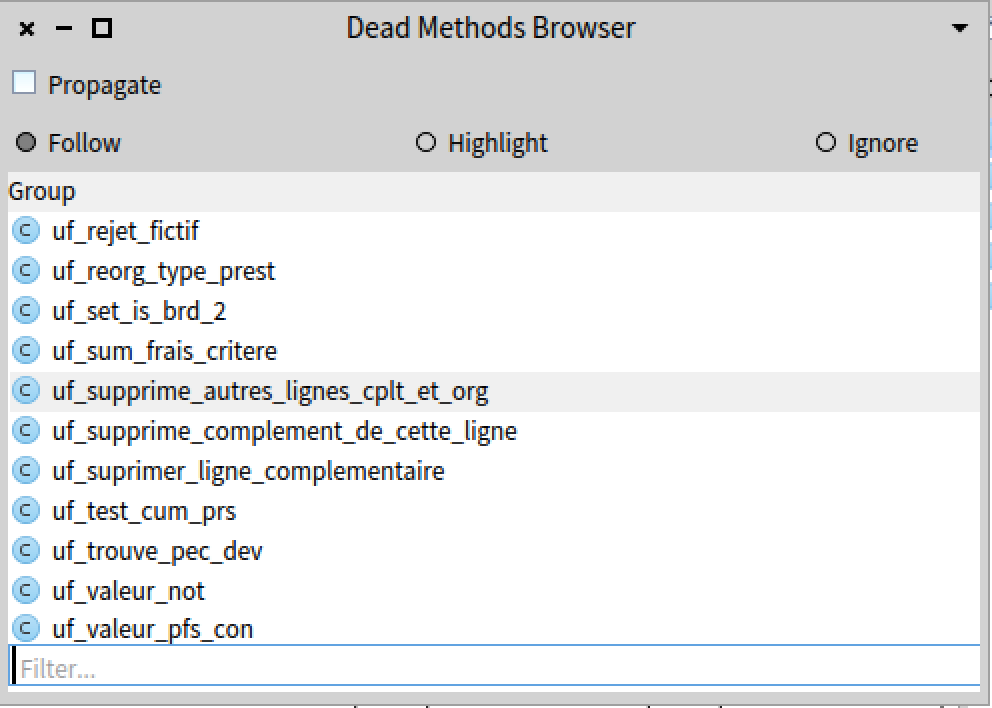
\includegraphics[width=0.5\textwidth]{./figures/deadMethodBrowser.png}
  \caption{navigateurde code mort}
  \label{fig:deadMethodBrowser}
\end{center}
\vspace{-0.3cm}
\end{figure}
La \figref{deadMethodBrowser} montre le navigateur de code mort.
Ce navigateur pressent pour le moment les methods de l'entité courant du navigateur qui le sont jamais appelé dans le système et les que ces methods appels.

\subsubsection{navigateur de code dupliqué}
\begin{figure}[htbp]
  \begin{center}
  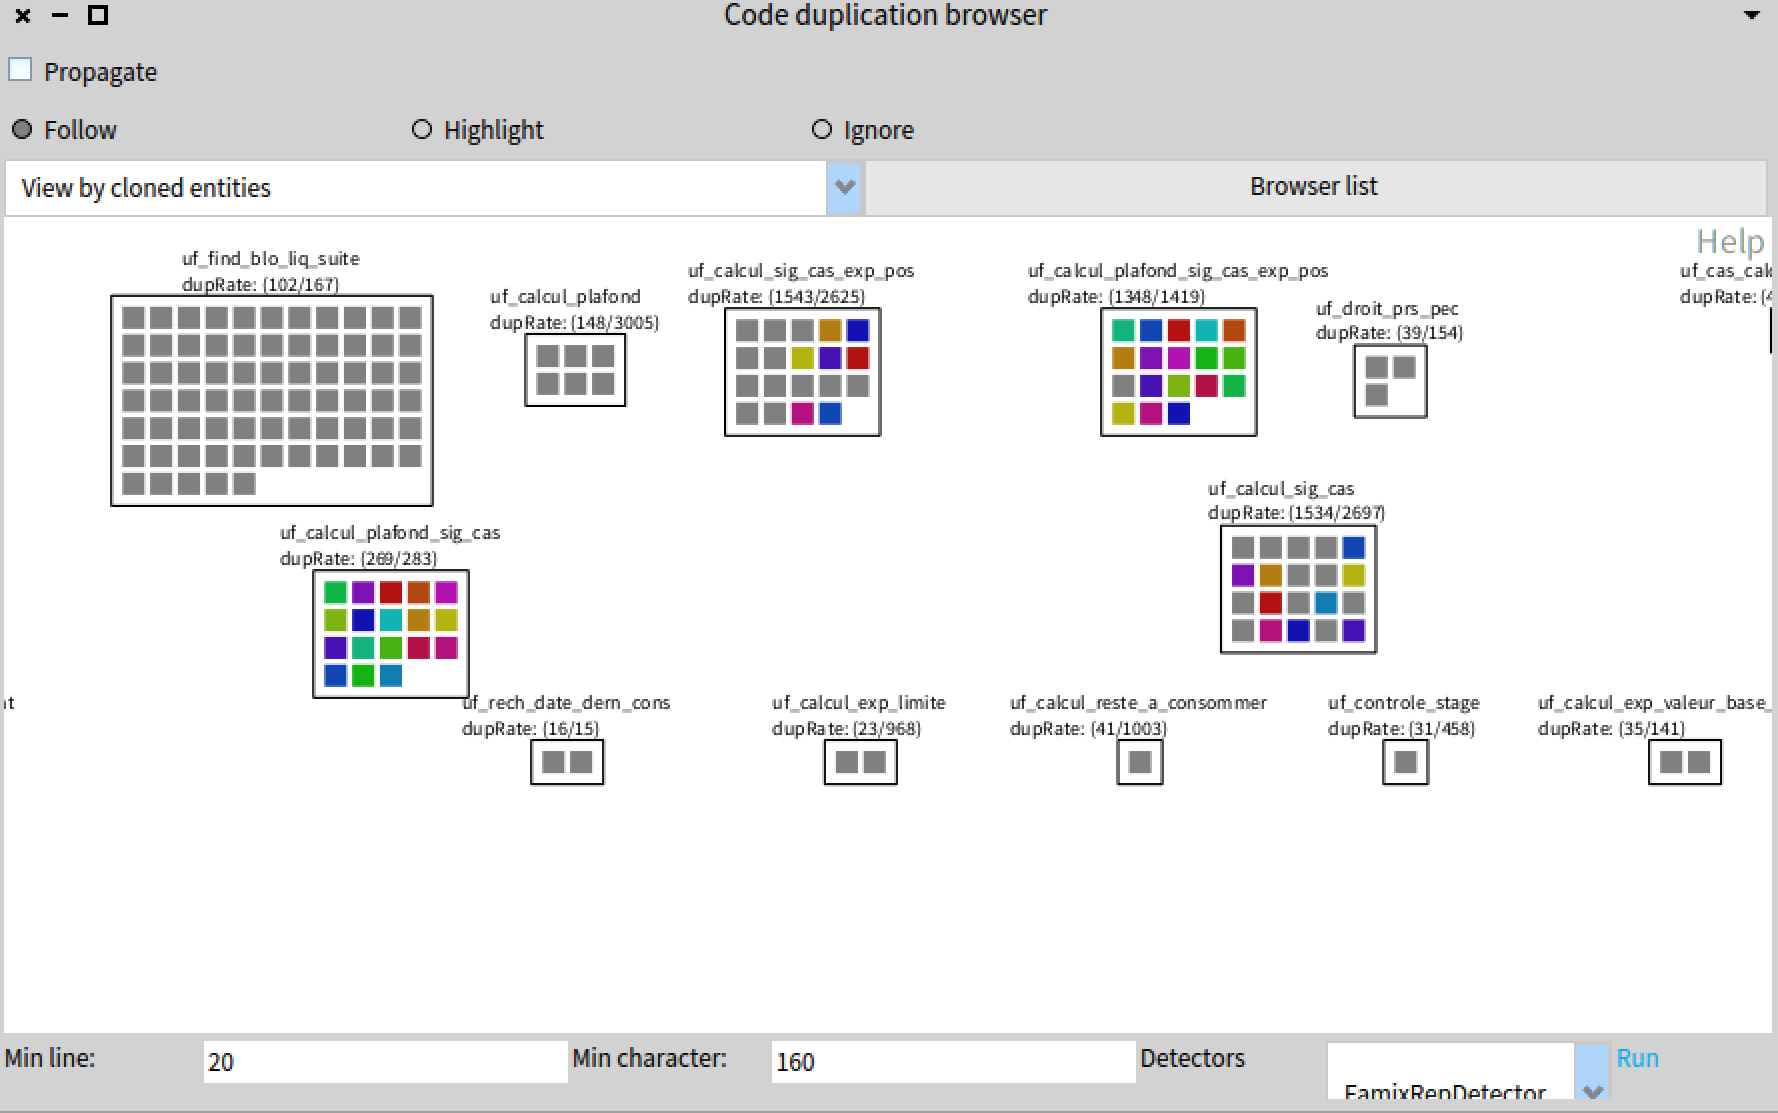
\includegraphics[width=0.7\textwidth]{./figures/duplicationBrowser.png}
  \caption{navigateur de code dupliqué}
  \label{fig:duplicationBrowser}
\end{center}
\vspace{-0.3cm}
\end{figure}
La \figref{duplicationBrowser} présent le navigateur de code dupliqué. Les carrés externes reprensentent les entités qui presentent de clone.
Dans le cas de la \figref{duplicationBrowser} c'est des methods.  
Les carrés internes représentent les clones que presentent une entité.
Les code dupliqués sont representés de façon de ce que l'utilisateur puis facilement l'inspecter.
Il utilise actuellement un algorithme de détection basé sur l'égalité strict des chaines de carctères \citep{Duca99b}. 
Cet algorithme peut être remplacé par un algorithme plus sophistiqué pour détecter les doublons \citep{Roy07a}. 

Supposont deux entités \textit{e1} et \textit{e2} qui presentent de clones en commun.
Quand l'utilisateur clique sur \textit{e1}, les clone de \textit{e1} prennent des couleurs differentes.
Les clones que \textit{e1} à en commun avec \textit{e2}, dans \textit{e2} prennent les mêmes couleurs que leurs que leurs semblables dans \textit{e1}.
Cela permet de voir plus facilement quel entités on de code en commun et de comparer les codes sources dans le navigateur de code que je presenterai dans la suite. 

\subsubsection{Navigateur de code source}

\begin{figure}[htbp]
  \begin{center}
  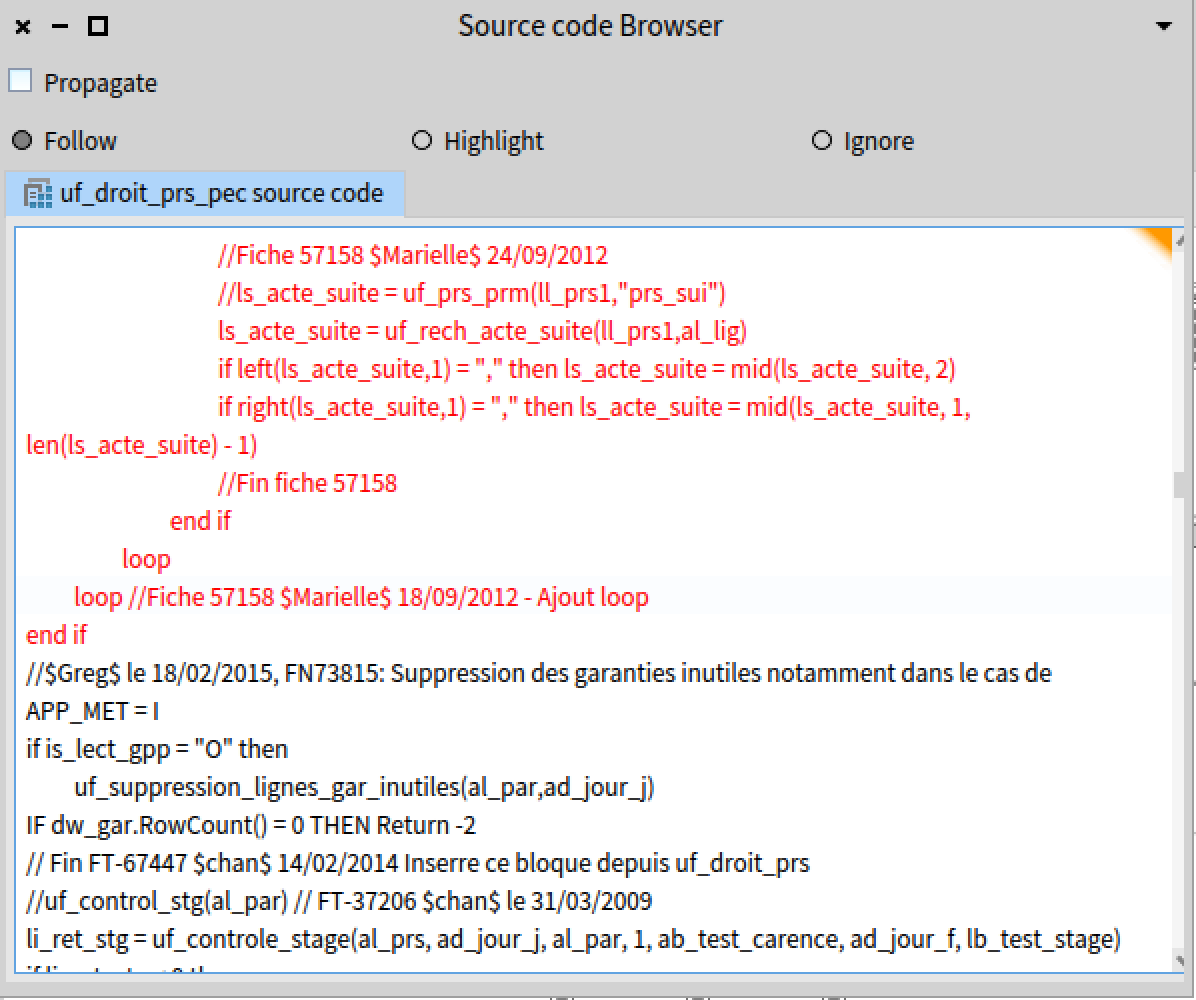
\includegraphics[width=0.7\textwidth]{./figures/sourceCodeBrowser.png}
  \caption{navigateur de code dupliqué}
  \label{fig:sourceCodeBrowser}
\end{center}
\vspace{-0.3cm}
\end{figure}
La \figref{sourceCodeBrowser} presente le navigateur de code source. 
Ce navigateur est une fenêtre qui affiche le code source de entité courant.
En particulier dans le cadre d'un fragment dupliqué, le code source de l'entité qui contient ce fragment est affiché normalement sauf que la partie du code qui represente le fragment dupliqué est en rouge 
comme sur la \figref{sourceCodeBrowser}

\section{Future traveaux}
\label{sec:roadmap}
Toutes les outils presentés ci-dessus sont conçus dans le but de netoyer le code de visualiser l'interaction entre les differentes classe de Izy Protect.
Par contre les developpeurs ne l'ont pas encore utilisés dans leurs quotidien.
Dans ce sens, j'identifie la validation de ces outils dans la suite mes traveaux.

D'un autre côté, l'entreprise prevoit de migrer une partie du système dans une architecture orienté service. 
Les développeurs ont donc exprémé le besoin d'extraire des règles metier du code.
Plusieurs traveaux sont presenter dans la literature dans ce sens en particulier  \cite{Lei05a} qui se base sur l'analyse static des interaction des fonctions avec les variables pour extraire les regles metier. 
Je souhaite combiner cette method avec  la method proposer \cite{anqu19a} pour propose un outil d'extraction de regles metier dans les systèmes patrimoniaux.

Je mettrai en place et j'etudirai  l'impact du DevOps a la CIM. 

\section{Publications}

Cette section présente la liste des  soumissions liée à cette thèse.

\begin{enumerate}
  \item Journée de travail du groupe Rimel du GR/GPL: HOUEKPETODJI Honoré, Nicolas Anquetil
  \textit{Improving practices in a medium Franch company: First step}
  \item 13th International Conference on the Quality of Information and Communications Technology 2020: HOUEKPETODJI Honoré,
  
\end{enumerate}

\section{Formation doctorale}


\section{Projet professionnel}



\footnotesize{
  %\bibliographystyle{alpha}
  % natbib 
 \bibliographystyle{plainnat}
\bibliography{rmod,others}
}

\end{document}